\documentclass[polish,a4paper]{article}
\usepackage[T1]{fontenc}
\usepackage{lmodern}
\usepackage[utf8]{inputenc}
\usepackage[polish]{babel}
\usepackage{tikz}
    \usetikzlibrary{
        arrows,
        shadows,
        shapes
    }
\usepackage{pgfplots}
\usepackage[margin = 1.in]{geometry}
\usepackage{subcaption}
\usepackage[export]{adjustbox}
\usepackage{hyperref}
\usepackage{tabularx}
\usepackage{mathtools}
\usepackage{multirow}
\usepackage{graphicx}
\usepackage{array}
\usepackage{hhline}
\usepackage{pdflscape}
\usepackage{url}
\usepackage{filecontents}
\usepackage{float}
\usepackage{csvsimple}
\usepackage{booktabs}
\usepackage{makecell}

\pgfplotsset{compat=1.18}

\newcommand{\name}[1]{\sffamily\bfseries\scriptsize #1}

\newcommand{\frontpage}[6]{
    \noindent
    \begin{tabularx}{\textwidth}{@{}X@{}l@{}}
        \begin{tabular}[t]{||m{0.5\textwidth}|m{0.25\textwidth}||}
            \hhline{|t:==:t|}
            \multicolumn{2}{||c||}{}\\
            \multicolumn{2}{||c||}{{\LARGE #1}}\\
            \multicolumn{2}{||c||}{}\\
            \hhline{||--||}
            \name{Kierunek} & \name{Termin}\\
            \textit{#2} & \textit{#3} \\
            \hhline{||--||}
            \name{Imię, nazwisko, numer albumu} & \name{Data}\\
            \textit{#4} & \textit{#5} \\
            \hhline{||--||}
            \multicolumn{2}{||l||}{\name{Link do projektu}} \\
            \multicolumn{2}{||l||}{\url{#6}} \\
            \hhline{|b:==:b|}
        \end{tabular}
        &
        
\includegraphics[width=2.25cm,valign=T]{PWr.png}
    \end{tabularx}
    \vspace{.5cm}
    
    \begin{center}
        \LARGE \textsc{Raport}
    \end{center}
    
    \noindent\rule[0.5cm]{\textwidth}{1pt}
}

\begin{document}
\frontpage{Projektowanie i analiza algorytmów}{Informatyczne Systemy Automatyki}{czwartek 11:15}{Iwo Chwiszczuk 280043}{\today}{https://github.com/iwonieevo/Sorting-algorithms}

\begin{center}
    \Large\textrm{Implementacja i Analiza Algorytmów Sortowania}
\end{center}

\begin{figure}[h]
	\centering
	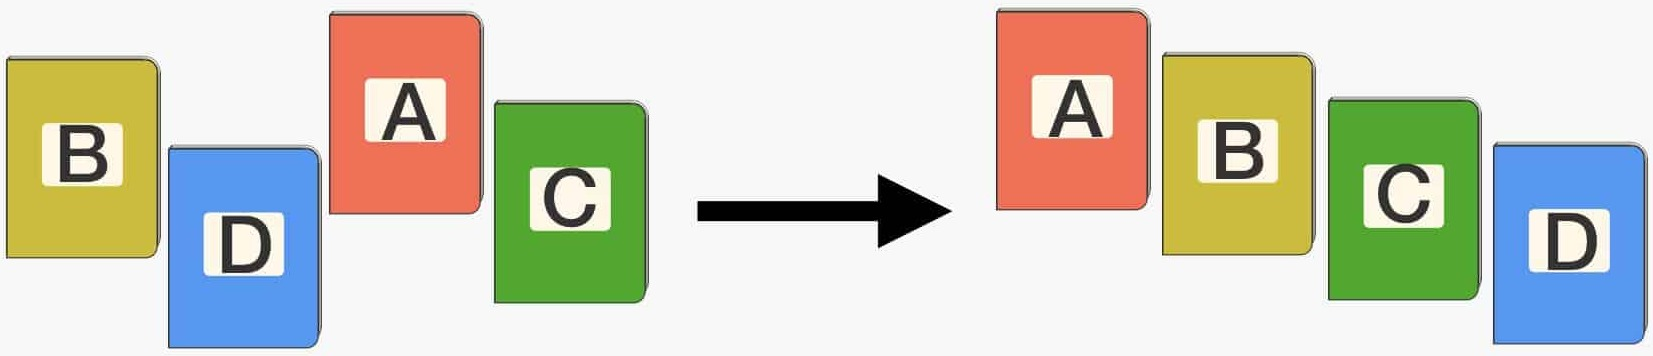
\includegraphics[width=\linewidth]{Sorting-algorithm.jpg}
\end{figure}

\newpage
\renewcommand{\figurename}{Wykres}
\renewcommand{\listfigurename}{Spis wykresów}
\tableofcontents
\listoftables
\listoffigures

\newpage
\section{Streszczenie}
Celem projektu była implementacja wybranych algorytmów sortowania oraz analiza ich złożoności czasowej. Zbadano trzy metody: MergeSort (sortowanie przez scalanie), QuickSort (sortowanie szybkie) oraz IntroSort (sortowanie introspektywne). Najbardziej wydajnym algorytmem spośród badanych okazał się IntroSort. QuickSort może osiągać wysoką wydajność dla określonych danych, lecz jego czas wykonania bywa niestabilny. MergeSort jest zazwyczaj wolniejszy, ale zapewnia stabilność wykonania oraz stabilność sortowania (zachowanie kolejności elementów równych).

\section{Wstęp}
\subsection{Opis problemu sortowania}
Sortowanie to jedno z fundamentalnych zagadnień informatyki, które ma kluczowe znaczenie w optymalizacji wielu procesów obliczeniowych. Polega na uporządkowaniu zbioru danych według określonego kryterium, np. wartości liczbowych lub kolejności alfabetycznej. Jest to kluczowy problem występujący w wielu obszarach, takich jak bazy danych, algorytmy wyszukiwania czy przetwarzanie dużych zbiorów danych.

\subsection{Klasyfikacja algorytmów sortowania}
Algorytmy sortowania można klasyfikować według różnych kryteriów, m.in.:
\begin{itemize}
    \item \textbf{Złożoność obliczeniowa} – określa liczbę operacji wykonywanych przez algorytm w zależności od liczby elementów wejściowych. Rozróżnia się przypadek optymistyczny, pesymistyczny oraz średni.
    \item \textbf{Zużycie pamięci} – określa ilość dodatkowej pamięci wymaganej do wykonania algorytmu w zależności od rozmiaru danych wejściowych.
    \item \textbf{Rekurencyjność} – algorytm może być implementowany w sposób rekurencyjny lub iteracyjny.
    \item \textbf{Stabilność} – algorytm jest stabilny, jeśli zachowuje kolejność względną elementów o równych wartościach klucza.
\end{itemize}

Istnieją również inne klasyfikacje, jednak w tym projekcie analiza skupia się głównie na złożoności obliczeniowej, a w szczególności na czasie wykonania badanych algorytmów.

\subsection{Badane algorytmy sortowania}
\subsubsection{MergeSort}
\begin{itemize}
	\item{MergeSort to algorytm sortowania wykorzystujący strategię dziel i rządź \textit{(divide and conquer)}. Polega na rekurencyjnym (lub iteracyjnym) dzieleniu tablicy na mniejsze podtablice, sortowaniu ich, a następnie scalaniu (\texttt{merge}) w sposób uporządkowany.}
	\item{Pesymistyczna, średnia oraz optymistyczna złożoność wynosi $O(n \ \log_2 n)$ - algorytm zawsze dzieli sortowaną tablicę na $\log_2 n$ poziomów i na każdym wykonuje $O(n)$ operacji scalania.}
	\item{Merge Sort wymaga dodatkowej pamięci o złożoności $O(n)$, ponieważ przechowuje tymczasowe kopie scalanych podtablic. W wersji rekurencyjnej dodatkowo wykorzystywany jest stos rekurencyjny o złożoności $O(\log_2 n)$, ponieważ głębokość rekurencji odpowiada liczbie poziomów podziału tablicy. W wersji iteracyjnej zużycie dodatkowej pamięci jest ograniczone do pamięci wymaganej na tymczasowe kopie podtablic.}
	\item{Algorytm jest stabilny, czyli elementy o jednakowej wartości zachowują swoją pierwotną kolejność. \\
W ramach projektu zaimplementowano iteracyjną wersję MergeSort, która eliminuje stos rekurencyjny poprzez iteracyjne scalanie coraz większych fragmentów tablicy, co może poprawić wydajność w praktycznych zastosowaniach.}
\end{itemize}

\subsubsection{QuickSort}
\begin{itemize}
	\item{QuickSort to algorytm sortowania wykorzystujący strategię dziel i rządź. Polega na rekurencyjnym (lub iteracyjnym) podziale tablicy na mniejsze podtablice względem wybranego elementu zwanego pivotem, a następnie sortowaniu każdej z nich oddzielnie. Podział odbywa się w taki sposób, że elementy mniejsze od pivota są umieszczane po jego lewej stronie, a większe po prawej. Proces ten jest kontynuowany, aż podtablice będą miały tylko jeden element.}
	\item{Pesymistyczna złożoność QuickSort wynosi $O(n^2)$, co występuje, gdy pivot dzieli tablicę w sposób bardzo nierównomierny (np. zawsze wybierany jest największy lub najmniejszy element). W średnim i optymistycznym przypadku algorytm działa w czasie $O(n \ \log_2 n)$, co jest związane z równomiernym podziałem tablicy.}
	\item{QuickSort działa w miejscu (in-place), co oznacza, że nie wymaga dodatkowej pamięci poza stosową rekurencją lub pomocniczymi strukturami dla implementacji iteracyjnej. Złożoność pamięciowa wynosi $O(\log_2 n)$ w typowych przypadkach, ponieważ głębokość rekurencji (lub liczba przechowywanych zakresów w wersji iteracyjnej) jest ograniczona do liczby poziomów podziału. W pesymistycznym przypadku może wzrosnąć do $O(n)$, jeśli podziały są skrajnie nierównomierne.}
	\item{Algorytm nie jest stabilny, ponieważ podczas podziału tablicy może zmieniać względną kolejność elementów o tej samej wartości.}
	\item{W ramach projektu zaimplementowano iteracyjną wersję QuickSort, eliminującą stos rekurencyjny poprzez zarządzanie zakresami podtablic w pętli. Jako pivot wybrano medianę trzech elementów (pierwszego, środkowego i ostatniego), co poprawia równomierność podziału i stabilizuje wydajność algorytmu.}
\end{itemize}

\subsubsection{IntroSort}
\begin{itemize}
	\item{IntroSort to algorytm sortowania łączący zalety QuickSort, HeapSort (sortowanie przez kopcowanie) i InsertionSort (sortowanie przez wstawianie), co pozwala na uzyskanie optymalnej wydajności zarówno w przypadku danych posortowanych, jak i silnie nieuporządkowanych. Wykorzystuje strategię dziel i rządź, a jego kluczową cechą jest monitorowanie głębokości rekurencji, aby unikać pesymistycznej złożoności $O(n^2)$. Algorytm rozpoczyna działanie jako QuickSort, wykorzystując podział tablicy wokół pivota i rekurencyjne sortowanie podtablic. Jeśli głębokość rekurencji przekroczy ustalony próg $2 \log_2 n$, algorytm przełącza się na HeapSort, który gwarantuje $O(n \ \log_2 n)$ w najgorszym przypadku. Dodatkowo, dla bardzo małych tablic (zwykle poniżej 16 elementów) stosowany jest InsertionSort, który działa wydajnie dla małych zbiorów danych.}
	\item{Pesymistyczna, średnia oraz optymistyczna złożoność czasowa IntroSort wynosi $O(n \ \log_2 n)$. Dzięki adaptacyjnemu podejściu algorytm unika problemu degeneracji występującego w QuickSort, gdzie nierównomierne podziały mogą prowadzić do złożoności $O(n^2)$.}
	\item{IntroSort działa w miejscu i ma złożoność pamięciową $O(\log_2 n)$, wynikającą z rekurencyjnej implementacji QuickSort w początkowej fazie. Algorytm nie jest stabilny, ponieważ HeapSort może zmieniać względną kolejność elementów o tej samej wartości.}
	\item{W ramach projektu zaimplementowano wersję IntroSort, która wykorzystuje QuickSort jako podstawową metodę sortowania, monitorując głębokość rekurencji. Jeśli liczba podziałów przekroczy $2 \log_2 n$, algorytm przełącza się na HeapSort. Dodatkowo, dla podtablic mniejszych niż 16 elementów stosowany jest InsertionSort, co poprawia wydajność dla niewielkich zbiorów danych.}
\end{itemize}

\newpage
\section{Eksperymenty i analiza wyników}
\subsection{Metodyka eksperymentów}
Badania zostały przeprowadzone w pliku \texttt{main.cpp}, w głównej pętli programu. Na początku znajdują się deklaracje użytych funkcji:

\begin{itemize} 
    \item \texttt{fit\_nlogn} — dopasowuje współczynniki $A$ i $B$ funkcji regresji $f(n) = A \cdot n \log_2 n + B$ do danych \texttt{data}, odpowiadającym wartościom \texttt{sizes}, przy użyciu metody najmniejszych kwadratów.
    \item \texttt{generate\_random\_data} — służy do zapełniania tablicy (wskaźnik na nią przekazywany jest jako parametr) pseudolosowymi liczbami całkowitymi z określonego zakresu. Do generowania danych użyto biblioteki \texttt{random}. Dodatkowo przekazywany jest parametr \texttt{percentage}, określający procent początkowych elementów, które mają być posortowane. Wartość ujemna oznacza, że wskazany procent elementów będzie posortowany w kolejności odwrotnej. Do wstępnego posortowania, wykorzystano własną implementację \texttt{IntroSort}.
    \item \texttt{measure\_sorting\_time} — mierzy czas wykonywania funkcji sortującej. Wszystkie algorytmy przyjmują jako parametry:
        \begin{enumerate}
            \item wskaźnik na tablicę do posortowania,
            \item indeks elementu, od którego ma się rozpocząć sortowanie,
            \item indeks elementu, na którym ma się zakończyć sortowanie.
        \end{enumerate} 
        Czyli jeśli chcemy posortować całą tablicę, należy przekazać 0 jako drugi parametr i \texttt{rozmiar}-1 jako trzeci. Do pomiaru czasu wykorzystano bibliotekę \texttt{chrono}, a funkcja zwraca czas wykonania w nanosekundach.
\end{itemize}

W pętli głównej programu określono rozmiary tablic do przetestowania, zakres wartości losowych oraz stopień wstępnego posortowania. Dla każdego algorytmu, rozmiaru tablicy i poziomu uporządkowania danych przeprowadzana jest seria pomiarów. Dla każdej kombinacji parametrów pętlę powtórzono \texttt{N\_TIMES} razy (w eksperymencie przyjęto wartość 100).

Aby zapewnić spójność wyników, na początku tworzona jest referencyjna tablica z wygenerowanymi danymi. Następnie dla każdego pomiaru tworzona jest jej kopia, która dopiero podlega sortowaniu. Zmierzony czas jest dodawany do odpowiedniego elementu tablicy przechowującej wyniki. Po wykonaniu \texttt{N\_TIMES} pomiarów, wartość każdej komórki podzielono przez \texttt{N\_TIMES}, co pozwala uzyskać średni czas działania algorytmu. Ostateczne wyniki są zapisywane, a tablica wyników wyzerowana przed kolejnym pomiarem.

Dane do dalszej analizy zostały zapisane do pliku \texttt{results.csv}, który znajduje się w repozytorium.

\subsection{Wyniki testów}
Na kolejnych stronach przedstawiono wyniki testów w formie tabel i wykresów. Dla każdego algorytmu stworzono:

\begin{itemize} 
    \item Tabelę ze średnimi czasami wykonywania, w zależności od typu danych wejściowych. 
    \item Dwa wykresy porównujące czasy działania — jeden w skali standardowej, drugi w skali $\log x$-$\log y$ (Wraz z dopasowaniami do O($n \ \log n$) - przerywaną linią).
\end{itemize}

Dodatkowo porównano algorytmy między sobą, przedstawiając wyniki na wykresach liniowych — również w dwóch wersjach: standardowej i $\log x$-$\log y$.

\newpage

\newcolumntype{C}[1]{>{\centering\arraybackslash}p{#1}}

\begin{table}[H]
    \centering
    \caption{Wyniki - MergeSort}
    \label{tab:merge_sort}
    \resizebox{\textwidth}{!}{
    \begin{tabular}{|C{1.4cm}|*{7}{C{1.6cm}|}C{1.8cm}|}
        \hline
        \multirow{2}{*}{\textbf{Rozmiar}} & \multicolumn{7}{c|}{\textbf{Liczba posortowanych elementów tablicy}} & \multirow{2}{*}{\textbf{\makecell{Odwrotna\\kolejność}}} \\
        \cline{2-8}
        & \textbf{0\%} & \textbf{25\%} & \textbf{50\%} & \textbf{75\%} & \textbf{95\%} & \textbf{99\%} & \textbf{99.7\%} & \\
        \hline
        \csvreader[
        head to column names,
        late after line=\\ \hline,
        late after last line=\\ \hline
        ]{../results.csv}{}{\SIZE & \csvcolii & \csvcoliii & \csvcoliv & \csvcolv & \csvcolvi & \csvcolvii & \csvcolviii & \csvcolix}
    \end{tabular}
    }
\end{table}

\begin{table}[H]
    \centering
    \caption{Wyniki - QuickSort}
    \label{tab:quick_sort}
    \resizebox{\textwidth}{!}{
    \begin{tabular}{|C{1.4cm}|*{7}{C{1.6cm}|}C{1.8cm}|}
        \hline
        \multirow{2}{*}{\textbf{Rozmiar}} & \multicolumn{7}{c|}{\textbf{Liczba posortowanych elementów tablicy}} & \multirow{2}{*}{\textbf{\makecell{Odwrotna\\kolejność}}} \\
        \cline{2-8}
        & \textbf{0\%} & \textbf{25\%} & \textbf{50\%} & \textbf{75\%} & \textbf{95\%} & \textbf{99\%} & \textbf{99.7\%} & \\
        \hline
        \csvreader[
        head to column names,
        late after line=\\ \hline,
        late after last line=\\ \hline
        ]{../results.csv}{}{\SIZE & \csvcolx & \csvcolxi & \csvcolxii & \csvcolxiii & \csvcolxiv & \csvcolxv & \csvcolxvi & \csvcolxvii}
    \end{tabular}
    }
\end{table}

\begin{table}[H]
    \centering
    \caption{Wyniki - IntroSort}
    \label{tab:intro_sort}
    \resizebox{\textwidth}{!}{
    \begin{tabular}{|C{1.4cm}|*{7}{C{1.6cm}|}C{1.8cm}|}
        \hline
        \multirow{2}{*}{\textbf{Rozmiar}} & \multicolumn{7}{c|}{\textbf{Liczba posortowanych elementów tablicy}} & \multirow{2}{*}{\textbf{\makecell{Odwrotna\\kolejność}}} \\
        \cline{2-8}
        & \textbf{0\%} & \textbf{25\%} & \textbf{50\%} & \textbf{75\%} & \textbf{95\%} & \textbf{99\%} & \textbf{99.7\%} & \\
        \hline
        \csvreader[
        head to column names,
        late after line=\\ \hline,
        late after last line=\\ \hline
        ]{../results.csv}{}{\SIZE & \csvcolxviii & \csvcolxix & \csvcolxx & \csvcolxxi & \csvcolxxii & \csvcolxxiii & \csvcolxxiv & \csvcolxxv}
    \end{tabular}
    }
\end{table}

\newpage

%MergeSort
\begin{figure}[H]
    \centering
    \begin{tikzpicture}
        \begin{axis}[width=\textwidth, height=0.6\textwidth, xlabel={Rozmiar danych \(n\)}, ylabel={Czas [ns]}, grid=both, title={Porównanie czasu działania MergeSort dla różnych typów danych wejściowych}, minor tick num=4,
        enlargelimits=0.05, legend cell align={left}, cycle list name=color list, legend style={at={(0.5,-0.15)}, anchor=north, legend columns=4, column sep=1ex}]
            % 0%
            \addplot[color=red, mark=*]
            table[col sep=comma, x=SIZE, y=MergeS-0] {../results.csv};
            \addlegendentry{MergeSort 0\%}

            \addplot[forget plot, color=red, dashed, domain=100:1000000, samples=1000] {7.84876*x*log2(x)+370790};

            % 25%
            \addplot[color=blue, mark=*]
            table[col sep=comma, x=SIZE, y=MergeS-25] {../results.csv};
            \addlegendentry{MergeSort 25\%}

            \addplot[forget plot, color=blue, dashed, domain=100:1000000, samples=1000] {7.1813*x*log2(x)+395242};

            % 50%
            \addplot[color=green, mark=*]
            table[col sep=comma, x=SIZE, y=MergeS-50] {../results.csv};
            \addlegendentry{MergeSort 50\%}

            \addplot[forget plot, color=green, dashed, domain=100:1000000, samples=1000] {6.42042*x*log2(x)+384042};

            % 75%
            \addplot[color=orange, mark=*]
            table[col sep=comma, x=SIZE, y=MergeS-75] {../results.csv};
            \addlegendentry{MergeSort 75\%}

            \addplot[forget plot, color=orange, dashed, domain=100:1000000, samples=1000] {5.66871*x*log2(x)+370258};

            % 95%
            \addplot[color=purple, mark=*]
            table[col sep=comma, x=SIZE, y=MergeS-95] {../results.csv};
            \addlegendentry{MergeSort 95\%}

            \addplot[forget plot, color=purple, dashed, domain=100:1000000, samples=1000] {5.05519*x*log2(x)+375628};

            % 99%
            \addplot[color=brown, mark=*]
            table[col sep=comma, x=SIZE, y=MergeS-99] {../results.csv};
            \addlegendentry{MergeSort 99\%}

            \addplot[forget plot, color=brown, dashed, domain=100:1000000, samples=1000] {4.94232*x*log2(x)+389375};
            
            % 99.7%
            \addplot[color=gray, mark=*]
            table[col sep=comma, x=SIZE, y=MergeS-997] {../results.csv};
            \addlegendentry{MergeSort 99.7\%}

            \addplot[forget plot, color=gray, dashed, domain=100:1000000, samples=1000] {4.92861*x*log2(x)+378928};
            
            % reverse
            \addplot[color=pink, mark=*]
            table[col sep=comma, x=SIZE, y=MergeS-reverse] {../results.csv};
            \addlegendentry{MergeSort reverse}

            \addplot[forget plot, color=pink, dashed, domain=100:1000000, samples=1000] {5.24058*x*log2(x)+330112};
        \end{axis}
    \end{tikzpicture}
    \caption{MergeSort}
    \label{fig:mergesort}
\end{figure}

\begin{figure}[H]
    \centering
    \begin{tikzpicture}
        \begin{axis}[width=\textwidth, height=0.6\textwidth, xlabel={Rozmiar danych \(n\)}, ylabel={Czas [ns]}, grid=both, title={Porównanie czasu działania MergeSort dla różnych typów danych wejściowych - $\log x$-$\log y$}, 
        enlargelimits=0.05, legend cell align={left}, cycle list name=color list, legend style={at={(0.5,-0.15)}, anchor=north, legend columns=4, column sep=1ex}, xmode=log, ymode=log]
            % 0%
            \addplot[color=red, mark=*]
            table[col sep=comma, x=SIZE, y=MergeS-0] {../results.csv};
            \addlegendentry{MergeSort 0\%}

            \addplot[forget plot, color=red, dashed, domain=100:1000000, samples=1000] {7.84876*x*log2(x)+370790};

            % 25%
            \addplot[color=blue, mark=*]
            table[col sep=comma, x=SIZE, y=MergeS-25] {../results.csv};
            \addlegendentry{MergeSort 25\%}

            \addplot[forget plot, color=blue, dashed, domain=100:1000000, samples=1000] {7.1813*x*log2(x)+395242};

            % 50%
            \addplot[color=green, mark=*]
            table[col sep=comma, x=SIZE, y=MergeS-50] {../results.csv};
            \addlegendentry{MergeSort 50\%}

            \addplot[forget plot, color=green, dashed, domain=100:1000000, samples=1000] {6.42042*x*log2(x)+384042};

            % 75%
            \addplot[color=orange, mark=*]
            table[col sep=comma, x=SIZE, y=MergeS-75] {../results.csv};
            \addlegendentry{MergeSort 75\%}

            \addplot[forget plot, color=orange, dashed, domain=100:1000000, samples=1000] {5.66871*x*log2(x)+370258};

            % 95%
            \addplot[color=purple, mark=*]
            table[col sep=comma, x=SIZE, y=MergeS-95] {../results.csv};
            \addlegendentry{MergeSort 95\%}

            \addplot[forget plot, color=purple, dashed, domain=100:1000000, samples=1000] {5.05519*x*log2(x)+375628};

            % 99%
            \addplot[color=brown, mark=*]
            table[col sep=comma, x=SIZE, y=MergeS-99] {../results.csv};
            \addlegendentry{MergeSort 99\%}

            \addplot[forget plot, color=brown, dashed, domain=100:1000000, samples=1000] {4.94232*x*log2(x)+389375};
            
            % 99.7%
            \addplot[color=gray, mark=*]
            table[col sep=comma, x=SIZE, y=MergeS-997] {../results.csv};
            \addlegendentry{MergeSort 99.7\%}

            \addplot[forget plot, color=gray, dashed, domain=100:1000000, samples=1000] {4.92861*x*log2(x)+378928};
            
            % reverse
            \addplot[color=pink, mark=*]
            table[col sep=comma, x=SIZE, y=MergeS-reverse] {../results.csv};
            \addlegendentry{MergeSort reverse}

            \addplot[forget plot, color=pink, dashed, domain=100:1000000, samples=1000] {5.24058*x*log2(x)+330112};
        \end{axis}
    \end{tikzpicture}
    \caption{MergeSort (w skali $\log x$-$\log y$)}
    \label{fig:mergesort-loglog}
\end{figure}

\newpage

%QuickSort
\begin{figure}[H]
    \centering
    \begin{tikzpicture}
        \begin{axis}[width=\textwidth, height=0.6\textwidth, xlabel={Rozmiar danych \(n\)}, ylabel={Czas [ns]}, grid=both, title={Porównanie czasu działania QuickSort dla różnych typów danych wejściowych}, minor tick num=4,
        enlargelimits=0.05, legend cell align={left}, cycle list name=color list, legend style={at={(0.5,-0.15)}, anchor=north, legend columns=4, column sep=1ex}]
            % 0%
            \addplot[color=red, mark=*]
            table[col sep=comma, x=SIZE, y=QuickS-0] {../results.csv};
            \addlegendentry{QuickSort 0\%}

            \addplot[forget plot, color=red, dashed, domain=100:1000000, samples=1000] {5.18494*x*log2(x)+273779};

            % 25%
            \addplot[color=blue, mark=*]
            table[col sep=comma, x=SIZE, y=QuickS-25] {../results.csv};
            \addlegendentry{QuickSort 25\%}

            \addplot[forget plot, color=blue, dashed, domain=100:1000000, samples=1000] {5.04143*x*log2(x)+283858};

            % 50%
            \addplot[color=green, mark=*]
            table[col sep=comma, x=SIZE, y=QuickS-50] {../results.csv};
            \addlegendentry{QuickSort 50\%}

            \addplot[forget plot, color=green, dashed, domain=100:1000000, samples=1000] {4.69657*x*log2(x)+289692};

            % 75%
            \addplot[color=orange, mark=*]
            table[col sep=comma, x=SIZE, y=QuickS-75] {../results.csv};
            \addlegendentry{QuickSort 75\%}

            \addplot[forget plot, color=orange, dashed, domain=100:1000000, samples=1000] {4.0559*x*log2(x)+266021};

            % 95%
            \addplot[color=purple, mark=*]
            table[col sep=comma, x=SIZE, y=QuickS-95] {../results.csv};
            \addlegendentry{QuickSort 95\%}

            \addplot[forget plot, color=purple, dashed, domain=100:1000000, samples=1000] {3.34507*x*log2(x)+190136};

            % 99%
            \addplot[color=brown, mark=*]
            table[col sep=comma, x=SIZE, y=QuickS-99] {../results.csv};
            \addlegendentry{QuickSort 99\%}

            \addplot[forget plot, color=brown, dashed, domain=100:1000000, samples=1000] {5.06594*x*log2(x)+-28961.5};
            
            % 99.7%
            \addplot[color=gray, mark=*]
            table[col sep=comma, x=SIZE, y=QuickS-997] {../results.csv};
            \addlegendentry{QuickSort 99.7\%}

            \addplot[forget plot, color=gray, dashed, domain=100:1000000, samples=1000] {9.92135*x*log2(x)+346537};
            
            % reverse
            \addplot[color=pink, mark=*]
            table[col sep=comma, x=SIZE, y=QuickS-reverse] {../results.csv};
            \addlegendentry{QuickSort reverse}

            \addplot[forget plot, color=pink, dashed, domain=100:1000000, samples=1000] {1.82628*x*log2(x)+-91188};
        \end{axis}
    \end{tikzpicture}
    \caption{QuickSort}
    \label{fig:quicksort}
\end{figure}

\begin{figure}[H]
    \centering
    \begin{tikzpicture}
        \begin{axis}[width=\textwidth, height=0.6\textwidth, xlabel={Rozmiar danych \(n\)}, ylabel={Czas [ns]}, grid=both, title={Porównanie czasu działania QuickSort dla różnych typów danych wejściowych - $\log x$-$\log y$}, 
        enlargelimits=0.05, legend cell align={left}, cycle list name=color list, legend style={at={(0.5,-0.15)}, anchor=north, legend columns=4, column sep=1ex}, xmode=log, ymode=log]
            % 0%
            \addplot[color=red, mark=*]
            table[col sep=comma, x=SIZE, y=QuickS-0] {../results.csv};
            \addlegendentry{QuickSort 0\%}

            \addplot[forget plot, color=red, dashed, domain=100:1000000, samples=1000] {5.18494*x*log2(x)+273779};

            % 25%
            \addplot[color=blue, mark=*]
            table[col sep=comma, x=SIZE, y=QuickS-25] {../results.csv};
            \addlegendentry{QuickSort 25\%}

            \addplot[forget plot, color=blue, dashed, domain=100:1000000, samples=1000] {5.04143*x*log2(x)+283858};

            % 50%
            \addplot[color=green, mark=*]
            table[col sep=comma, x=SIZE, y=QuickS-50] {../results.csv};
            \addlegendentry{QuickSort 50\%}

            \addplot[forget plot, color=green, dashed, domain=100:1000000, samples=1000] {4.69657*x*log2(x)+289692};

            % 75%
            \addplot[color=orange, mark=*]
            table[col sep=comma, x=SIZE, y=QuickS-75] {../results.csv};
            \addlegendentry{QuickSort 75\%}

            \addplot[forget plot, color=orange, dashed, domain=100:1000000, samples=1000] {4.0559*x*log2(x)+266021};

            % 95%
            \addplot[color=purple, mark=*]
            table[col sep=comma, x=SIZE, y=QuickS-95] {../results.csv};
            \addlegendentry{QuickSort 95\%}

            \addplot[forget plot, color=purple, dashed, domain=100:1000000, samples=1000] {3.34507*x*log2(x)+190136};

            % 99%
            \addplot[color=brown, mark=*]
            table[col sep=comma, x=SIZE, y=QuickS-99] {../results.csv};
            \addlegendentry{QuickSort 99\%}

            \addplot[forget plot, color=brown, dashed, domain=100:1000000, samples=1000] {5.06594*x*log2(x)+-28961.5};
            
            % 99.7%
            \addplot[color=gray, mark=*]
            table[col sep=comma, x=SIZE, y=QuickS-997] {../results.csv};
            \addlegendentry{QuickSort 99.7\%}

            \addplot[forget plot, color=gray, dashed, domain=100:1000000, samples=1000] {9.92135*x*log2(x)+346537};
            
            % reverse
            \addplot[color=pink, mark=*]
            table[col sep=comma, x=SIZE, y=QuickS-reverse] {../results.csv};
            \addlegendentry{QuickSort reverse}

            \addplot[forget plot, color=pink, dashed, domain=100:1000000, samples=1000] {1.82628*x*log2(x)+-91188};
        \end{axis}
    \end{tikzpicture}
    \caption{QuickSort (w skali $\log x$-$\log y$)}
    \label{fig:quicksort-loglog}
\end{figure}

\newpage

%IntroSort
\begin{figure}[H]
    \centering
    \begin{tikzpicture}
        \begin{axis}[width=\textwidth, height=0.6\textwidth, xlabel={Rozmiar danych \(n\)}, ylabel={Czas [ns]}, grid=both, title={Porównanie czasu działania IntroSort dla różnych typów danych wejściowych}, minor tick num=4,
        enlargelimits=0.05, legend cell align={left}, cycle list name=color list, legend style={at={(0.5,-0.15)}, anchor=north, legend columns=4, column sep=1ex}]
            % 0%
            \addplot[color=red, mark=*]
            table[col sep=comma, x=SIZE, y=IntroS-0] {../results.csv};
            \addlegendentry{IntroSort 0\%}

            \addplot[forget plot, color=red, dashed, domain=100:1000000, samples=1000] {4.24605*x*log2(x)+73641.7};

            % 25%
            \addplot[color=blue, mark=*]
            table[col sep=comma, x=SIZE, y=IntroS-25] {../results.csv};
            \addlegendentry{IntroSort 25\%}

            \addplot[forget plot, color=blue, dashed, domain=100:1000000, samples=1000] {4.11038*x*log2(x)+94075};

            % 50%
            \addplot[color=green, mark=*]
            table[col sep=comma, x=SIZE, y=IntroS-50] {../results.csv};
            \addlegendentry{IntroSort 50\%}

            \addplot[forget plot, color=green, dashed, domain=100:1000000, samples=1000] {3.75533*x*log2(x)+107965};

            % 75%
            \addplot[color=orange, mark=*]
            table[col sep=comma, x=SIZE, y=IntroS-75] {../results.csv};
            \addlegendentry{IntroSort 75\%}

            \addplot[forget plot, color=orange, dashed, domain=100:1000000, samples=1000] {3.08756*x*log2(x)+118736};

            % 95%
            \addplot[color=purple, mark=*]
            table[col sep=comma, x=SIZE, y=IntroS-95] {../results.csv};
            \addlegendentry{IntroSort 95\%}

            \addplot[forget plot, color=purple, dashed, domain=100:1000000, samples=1000] {2.94287*x*log2(x)+291939};

            % 99%
            \addplot[color=brown, mark=*]
            table[col sep=comma, x=SIZE, y=IntroS-99] {../results.csv};
            \addlegendentry{IntroSort 99\%}

            \addplot[forget plot, color=brown, dashed, domain=100:1000000, samples=1000] {4.21744*x*log2(x)+100245};
            
            % 99.7%
            \addplot[color=gray, mark=*]
            table[col sep=comma, x=SIZE, y=IntroS-997] {../results.csv};
            \addlegendentry{IntroSort 99.7\%}

            \addplot[forget plot, color=gray, dashed, domain=100:1000000, samples=1000] {4.80413*x*log2(x)+50491};
            
            % reverse
            \addplot[color=pink, mark=*]
            table[col sep=comma, x=SIZE, y=IntroS-reverse] {../results.csv};
            \addlegendentry{IntroSort reverse}

            \addplot[forget plot, color=pink, dashed, domain=100:1000000, samples=1000] {0.92977*x*log2(x)+-58047.9};
        \end{axis}
    \end{tikzpicture}
    \caption{IntroSort}
    \label{fig:introsort}
\end{figure}

\begin{figure}[H]
    \centering
    \begin{tikzpicture}
        \begin{axis}[width=\textwidth, height=0.6\textwidth, xlabel={Rozmiar danych \(n\)}, ylabel={Czas [ns]}, grid=both, title={Porównanie czasu działania IntroSort dla różnych typów danych wejściowych - $\log x$-$\log y$},
        enlargelimits=0.05, legend cell align={left}, cycle list name=color list, legend style={at={(0.5,-0.15)}, anchor=north, legend columns=4, column sep=1ex}, xmode=log, ymode=log]
            % 0%
            \addplot[color=red, mark=*]
            table[col sep=comma, x=SIZE, y=IntroS-0] {../results.csv};
            \addlegendentry{IntroSort 0\%}

            \addplot[forget plot, color=red, dashed, domain=100:1000000, samples=1000] {4.24605*x*log2(x)+73641.7};

            % 25%
            \addplot[color=blue, mark=*]
            table[col sep=comma, x=SIZE, y=IntroS-25] {../results.csv};
            \addlegendentry{IntroSort 25\%}

            \addplot[forget plot, color=blue, dashed, domain=100:1000000, samples=1000] {4.11038*x*log2(x)+94075};

            % 50%
            \addplot[color=green, mark=*]
            table[col sep=comma, x=SIZE, y=IntroS-50] {../results.csv};
            \addlegendentry{IntroSort 50\%}

            \addplot[forget plot, color=green, dashed, domain=100:1000000, samples=1000] {3.75533*x*log2(x)+107965};

            % 75%
            \addplot[color=orange, mark=*]
            table[col sep=comma, x=SIZE, y=IntroS-75] {../results.csv};
            \addlegendentry{IntroSort 75\%}

            \addplot[forget plot, color=orange, dashed, domain=100:1000000, samples=1000] {3.08756*x*log2(x)+118736};

            % 95%
            \addplot[color=purple, mark=*]
            table[col sep=comma, x=SIZE, y=IntroS-95] {../results.csv};
            \addlegendentry{IntroSort 95\%}

            \addplot[forget plot, color=purple, dashed, domain=100:1000000, samples=1000] {2.94287*x*log2(x)+291939};

            % 99%
            \addplot[color=brown, mark=*]
            table[col sep=comma, x=SIZE, y=IntroS-99] {../results.csv};
            \addlegendentry{IntroSort 99\%}

            \addplot[forget plot, color=brown, dashed, domain=100:1000000, samples=1000] {4.21744*x*log2(x)+100245};
            
            % 99.7%
            \addplot[color=gray, mark=*]
            table[col sep=comma, x=SIZE, y=IntroS-997] {../results.csv};
            \addlegendentry{IntroSort 99.7\%}

            \addplot[forget plot, color=gray, dashed, domain=100:1000000, samples=1000] {4.80413*x*log2(x)+50491};
            
            % reverse
            \addplot[color=pink, mark=*]
            table[col sep=comma, x=SIZE, y=IntroS-reverse] {../results.csv};
            \addlegendentry{IntroSort reverse}

            \addplot[forget plot, color=pink, dashed, domain=100:1000000, samples=1000] {0.92977*x*log2(x)+-58047.9};
        \end{axis}
    \end{tikzpicture}
    \caption{IntroSort (w skali $\log x$-$\log y$)}
    \label{fig:introsort-loglog}
\end{figure}

\newpage

%Porównanie
\begin{figure}[H]
    \centering
    \caption{Porównanie czasu działania algorytmów dla różnych typów danych wejściowych}
    \label{fig:comparison}
    \captionsetup[subfigure]{
        justification=justified,
        singlelinecheck=false,
        labelsep=space
    }
    \pgfplotsset{
        every axis/.style={
            width=\textwidth,
            height=3cm,
            scale only axis,
            grid=both,
            minor tick num=4,
            tick label style={font=\scriptsize},
            title style={
                yshift=2mm,
                align=center,
                font=\small
            },
            xlabel style={font=\scriptsize},
            ylabel style={font=\scriptsize},
            tick label style={font=\scriptsize},
            legend style={
                at={(0.5,-0.1)},
                anchor=north,
                legend columns=3,
                column sep=1ex,
                font=\scriptsize,
                draw=none
            },
            xlabel={Rozmiar danych \(n\)},
            ylabel={Czas [ns]},
            enlargelimits=0.05,
            legend cell align={left},
            cycle list name=color list
        }
    }
    
    \begin{subfigure}[b]{0.45\textwidth}
        \begin{tikzpicture}
            \begin{axis}[title={Porównanie czasu działania algorytmów dla\\0\% początkowych elementów posortowanych}]
                \addplot[color=red, mark=*]
                table[col sep=comma, x=SIZE, y=MergeS-0] {../results.csv};
                \addlegendentry{MergeSort}

                \addplot[color=blue, mark=*]
                table[col sep=comma, x=SIZE, y=QuickS-0] {../results.csv};
                \addlegendentry{QuickSort}

                \addplot[color=green, mark=*]
                table[col sep=comma, x=SIZE, y=IntroS-0] {../results.csv};
                \addlegendentry{IntroSort}
            \end{axis}
        \end{tikzpicture}
        \caption{0\% początkowych elementów posortowanych}
        \label{fig:comparison-0}
    \end{subfigure}
    \hspace{1.3cm}
    \begin{subfigure}[b]{0.45\textwidth}
        \begin{tikzpicture}
            \begin{axis}[title={Porównanie czasu działania algorytmów dla\\25\% początkowych elementów posortowanych}]
                \addplot[color=red, mark=*]
                table[col sep=comma, x=SIZE, y=MergeS-25] {../results.csv};
                \addlegendentry{MergeSort}

                \addplot[color=blue, mark=*]
                table[col sep=comma, x=SIZE, y=QuickS-25] {../results.csv};
                \addlegendentry{QuickSort}

                \addplot[color=green, mark=*]
                table[col sep=comma, x=SIZE, y=IntroS-25] {../results.csv};
                \addlegendentry{IntroSort}
            \end{axis}
        \end{tikzpicture}
        \caption{25\% początkowych elementów posortowanych}
        \label{fig:comparison-25}
    \end{subfigure}
    \vspace{0.5cm}
    \begin{subfigure}[b]{0.45\textwidth}
        \begin{tikzpicture}
            \begin{axis}[title={Porównanie czasu działania algorytmów dla\\50\% początkowych elementów posortowanych}]
                \addplot[color=red, mark=*]
                table[col sep=comma, x=SIZE, y=MergeS-50] {../results.csv};
                \addlegendentry{MergeSort}

                \addplot[color=blue, mark=*]
                table[col sep=comma, x=SIZE, y=QuickS-50] {../results.csv};
                \addlegendentry{QuickSort}

                \addplot[color=green, mark=*]
                table[col sep=comma, x=SIZE, y=IntroS-50] {../results.csv};
                \addlegendentry{IntroSort}
            \end{axis}
        \end{tikzpicture}
        \caption{50\% początkowych elementów posortowanych}
        \label{fig:comparison-50}
    \end{subfigure}
    \hspace{1.3cm}
    \begin{subfigure}[b]{0.45\textwidth}
        \begin{tikzpicture}
            \begin{axis}[title={Porównanie czasu działania algorytmów dla\\75\% początkowych elementów posortowanych}]
                \addplot[color=red, mark=*]
                table[col sep=comma, x=SIZE, y=MergeS-75] {../results.csv};
                \addlegendentry{MergeSort}

                \addplot[color=blue, mark=*]
                table[col sep=comma, x=SIZE, y=QuickS-75] {../results.csv};
                \addlegendentry{QuickSort}

                \addplot[color=green, mark=*]
                table[col sep=comma, x=SIZE, y=IntroS-75] {../results.csv};
                \addlegendentry{IntroSort}
            \end{axis}
        \end{tikzpicture}
        \caption{75\% początkowych elementów posortowanych}
        \label{fig:comparison-75}
    \end{subfigure}
    \vspace{0.5cm}
    \begin{subfigure}[b]{0.45\textwidth}
        \begin{tikzpicture}
            \begin{axis}[title={Porównanie czasu działania algorytmów dla\\95\% początkowych elementów posortowanych}]
                \addplot[color=red, mark=*]
                table[col sep=comma, x=SIZE, y=MergeS-95] {../results.csv};
                \addlegendentry{MergeSort}

                \addplot[color=blue, mark=*]
                table[col sep=comma, x=SIZE, y=QuickS-95] {../results.csv};
                \addlegendentry{QuickSort}

                \addplot[color=green, mark=*]
                table[col sep=comma, x=SIZE, y=IntroS-95] {../results.csv};
                \addlegendentry{IntroSort}
            \end{axis}
        \end{tikzpicture}
        \caption{95\% początkowych elementów posortowanych}
        \label{fig:comparison-95}
    \end{subfigure}
    \hspace{1.3cm}
    \begin{subfigure}[b]{0.45\textwidth}
        \begin{tikzpicture}
            \begin{axis}[title={Porównanie czasu działania algorytmów dla\\99\% początkowych elementów posortowanych}]
                \addplot[color=red, mark=*]
                table[col sep=comma, x=SIZE, y=MergeS-99] {../results.csv};
                \addlegendentry{MergeSort}

                \addplot[color=blue, mark=*]
                table[col sep=comma, x=SIZE, y=QuickS-99] {../results.csv};
                \addlegendentry{QuickSort}

                \addplot[color=green, mark=*]
                table[col sep=comma, x=SIZE, y=IntroS-99] {../results.csv};
                \addlegendentry{IntroSort}
            \end{axis}
        \end{tikzpicture}
        \caption{99\% początkowych elementów posortowanych}
        \label{fig:comparison-99}
    \end{subfigure}
    \vspace{0.5cm}
    \begin{subfigure}[b]{0.45\textwidth}
        \begin{tikzpicture}
            \begin{axis}[title={Porównanie czasu działania algorytmów dla\\99.7\% początkowych elementów posortowanych}]
                \addplot[color=red, mark=*]
                table[col sep=comma, x=SIZE, y=MergeS-997] {../results.csv};
                \addlegendentry{MergeSort}

                \addplot[color=blue, mark=*]
                table[col sep=comma, x=SIZE, y=QuickS-997] {../results.csv};
                \addlegendentry{QuickSort}

                \addplot[color=green, mark=*]
                table[col sep=comma, x=SIZE, y=IntroS-997] {../results.csv};
                \addlegendentry{IntroSort}
            \end{axis}
        \end{tikzpicture}
        \caption{99.7\% początkowych elementów posortowanych}
        \label{fig:comparison-997}
    \end{subfigure}
    \hspace{1.3cm}
    \begin{subfigure}[b]{0.45\textwidth}
        \begin{tikzpicture}
            \begin{axis}[title={Porównanie czasu działania algorytmów dla\\elementów posortowanych odwrotnie}]
                \addplot[color=red, mark=*]
                table[col sep=comma, x=SIZE, y=MergeS-reverse] {../results.csv};
                \addlegendentry{MergeSort}

                \addplot[color=blue, mark=*]
                table[col sep=comma, x=SIZE, y=QuickS-reverse] {../results.csv};
                \addlegendentry{QuickSort}

                \addplot[color=green, mark=*]
                table[col sep=comma, x=SIZE, y=IntroS-reverse] {../results.csv};
                \addlegendentry{IntroSort}
            \end{axis}
        \end{tikzpicture}
        \caption{Elementy posortowane odwrotnie}
        \label{fig:comparison-reverse}
    \end{subfigure}
\end{figure}

\newpage

\begin{figure}[H]
    \centering
    \caption{Porównanie czasu działania algorytmów dla różnych typów danych wejściowych - $\log x$-$\log y$}
    \label{fig:comparison-loglog}
    \captionsetup[subfigure]{
        justification=justified,
        singlelinecheck=false,
        labelsep=space
    }
    \pgfplotsset{
        every axis/.style={
            width=\textwidth,
            height=3cm,
            scale only axis,
            grid=both,
            ytick={1e2,1e3,1e4,1e5,1e6,1e7,1e8,1e9},
            tick label style={font=\scriptsize},
            title style={
                align=center,
                font=\small
            },
            xlabel style={font=\scriptsize},
            ylabel style={font=\scriptsize},
            tick label style={font=\scriptsize},
            legend style={
                at={(0.5,-0.15)},
                anchor=north,
                legend columns=3,
                column sep=1ex,
                font=\scriptsize,
                draw=none
            },
            xlabel={Rozmiar danych \(n\)},
            ylabel={Czas [ns]},
            enlargelimits=0.05,
            legend cell align={left},
            cycle list name=color list,
            xmode=log,
            ymode=log
        }
    }
    
    \begin{subfigure}[b]{0.45\textwidth}
        \begin{tikzpicture}
            \begin{axis}[title={Porównanie czasu działania algorytmów dla\\0\% początkowych elementów posortowanych}]
                \addplot[color=red, mark=*]
                table[col sep=comma, x=SIZE, y=MergeS-0] {../results.csv};
                \addlegendentry{MergeSort}

                \addplot[color=blue, mark=*]
                table[col sep=comma, x=SIZE, y=QuickS-0] {../results.csv};
                \addlegendentry{QuickSort}

                \addplot[color=green, mark=*]
                table[col sep=comma, x=SIZE, y=IntroS-0] {../results.csv};
                \addlegendentry{IntroSort}
            \end{axis}
        \end{tikzpicture}
        \caption{0\% początkowych elementów posortowanych}
        \label{fig:comparison-0-loglog}
    \end{subfigure}
    \hspace{1.3cm}
    \begin{subfigure}[b]{0.45\textwidth}
        \begin{tikzpicture}
            \begin{axis}[title={Porównanie czasu działania algorytmów dla\\25\% początkowych elementów posortowanych}]
                \addplot[color=red, mark=*]
                table[col sep=comma, x=SIZE, y=MergeS-25] {../results.csv};
                \addlegendentry{MergeSort}

                \addplot[color=blue, mark=*]
                table[col sep=comma, x=SIZE, y=QuickS-25] {../results.csv};
                \addlegendentry{QuickSort}

                \addplot[color=green, mark=*]
                table[col sep=comma, x=SIZE, y=IntroS-25] {../results.csv};
                \addlegendentry{IntroSort}
            \end{axis}
        \end{tikzpicture}
        \caption{25\% początkowych elementów posortowanych}
        \label{fig:comparison-25-loglog}
    \end{subfigure}
    \vspace{0.5cm}
    \begin{subfigure}[b]{0.45\textwidth}
        \begin{tikzpicture}
            \begin{axis}[title={Porównanie czasu działania algorytmów dla\\50\% początkowych elementów posortowanych}]
                \addplot[color=red, mark=*]
                table[col sep=comma, x=SIZE, y=MergeS-50] {../results.csv};
                \addlegendentry{MergeSort}

                \addplot[color=blue, mark=*]
                table[col sep=comma, x=SIZE, y=QuickS-50] {../results.csv};
                \addlegendentry{QuickSort}

                \addplot[color=green, mark=*]
                table[col sep=comma, x=SIZE, y=IntroS-50] {../results.csv};
                \addlegendentry{IntroSort}
            \end{axis}
        \end{tikzpicture}
        \caption{50\% początkowych elementów posortowanych}
        \label{fig:comparison-50-loglog}
    \end{subfigure}
    \hspace{1.3cm}
    \begin{subfigure}[b]{0.45\textwidth}
        \begin{tikzpicture}
            \begin{axis}[title={Porównanie czasu działania algorytmów dla\\75\% początkowych elementów posortowanych}]
                \addplot[color=red, mark=*]
                table[col sep=comma, x=SIZE, y=MergeS-75] {../results.csv};
                \addlegendentry{MergeSort}

                \addplot[color=blue, mark=*]
                table[col sep=comma, x=SIZE, y=QuickS-75] {../results.csv};
                \addlegendentry{QuickSort}

                \addplot[color=green, mark=*]
                table[col sep=comma, x=SIZE, y=IntroS-75] {../results.csv};
                \addlegendentry{IntroSort}
            \end{axis}
        \end{tikzpicture}
        \caption{75\% początkowych elementów posortowanych}
        \label{fig:comparison-75-loglog}
    \end{subfigure}
    \vspace{0.5cm}
    \begin{subfigure}[b]{0.45\textwidth}
        \begin{tikzpicture}
            \begin{axis}[title={Porównanie czasu działania algorytmów dla\\95\% początkowych elementów posortowanych}]
                \addplot[color=red, mark=*]
                table[col sep=comma, x=SIZE, y=MergeS-95] {../results.csv};
                \addlegendentry{MergeSort}

                \addplot[color=blue, mark=*]
                table[col sep=comma, x=SIZE, y=QuickS-95] {../results.csv};
                \addlegendentry{QuickSort}

                \addplot[color=green, mark=*]
                table[col sep=comma, x=SIZE, y=IntroS-95] {../results.csv};
                \addlegendentry{IntroSort}
            \end{axis}
        \end{tikzpicture}
        \caption{95\% początkowych elementów posortowanych}
        \label{fig:comparison-95-loglog}
    \end{subfigure}
    \hspace{1.3cm}
    \begin{subfigure}[b]{0.45\textwidth}
        \begin{tikzpicture}
            \begin{axis}[title={Porównanie czasu działania algorytmów dla\\99\% początkowych elementów posortowanych}]
                \addplot[color=red, mark=*]
                table[col sep=comma, x=SIZE, y=MergeS-99] {../results.csv};
                \addlegendentry{MergeSort}

                \addplot[color=blue, mark=*]
                table[col sep=comma, x=SIZE, y=QuickS-99] {../results.csv};
                \addlegendentry{QuickSort}

                \addplot[color=green, mark=*]
                table[col sep=comma, x=SIZE, y=IntroS-99] {../results.csv};
                \addlegendentry{IntroSort}
            \end{axis}
        \end{tikzpicture}
        \caption{99\% początkowych elementów posortowanych}
        \label{fig:comparison-99-loglog}
    \end{subfigure}
    \vspace{0.5cm}
    \begin{subfigure}[b]{0.45\textwidth}
        \begin{tikzpicture}
            \begin{axis}[title={Porównanie czasu działania algorytmów dla\\99.7\% początkowych elementów posortowanych}]
                \addplot[color=red, mark=*]
                table[col sep=comma, x=SIZE, y=MergeS-997] {../results.csv};
                \addlegendentry{MergeSort}

                \addplot[color=blue, mark=*]
                table[col sep=comma, x=SIZE, y=QuickS-997] {../results.csv};
                \addlegendentry{QuickSort}

                \addplot[color=green, mark=*]
                table[col sep=comma, x=SIZE, y=IntroS-997] {../results.csv};
                \addlegendentry{IntroSort}
            \end{axis}
        \end{tikzpicture}
        \caption{99.7\% początkowych elementów posortowanych}
        \label{fig:comparison-997-loglog}
    \end{subfigure}
    \hspace{1.3cm}
    \begin{subfigure}[b]{0.45\textwidth}
        \begin{tikzpicture}
            \begin{axis}[title={Porównanie czasu działania algorytmów dla\\elementów posortowanych odwrotnie}]
                \addplot[color=red, mark=*]
                table[col sep=comma, x=SIZE, y=MergeS-reverse] {../results.csv};
                \addlegendentry{MergeSort}

                \addplot[color=blue, mark=*]
                table[col sep=comma, x=SIZE, y=QuickS-reverse] {../results.csv};
                \addlegendentry{QuickSort}

                \addplot[color=green, mark=*]
                table[col sep=comma, x=SIZE, y=IntroS-reverse] {../results.csv};
                \addlegendentry{IntroSort}
            \end{axis}
        \end{tikzpicture}
        \caption{Elementy posortowane odwrotnie}
        \label{fig:comparison-reverse-loglog}
    \end{subfigure}
\end{figure}

\newpage

\subsection{Wnioski}
\subsubsection{Podsumowanie wyników}
Przeprowadzona analiza obejmuje porównanie czasów wykonywania algorytmów MergeSort, QuickSort oraz IntroSort w różnych przypadkach początkowego uporządkowania danych. Wyniki przedstawiają czas sortowania (w nanosekundach) dla różnych rozmiarów tablicy i stopni uporządkowania elementów.

\begin{itemize}
    \item{MergeSort zapewnia stabilne czasy wykonywania, lecz są one wyraźnie wyższe niż w przypadku pozostałych algorytmów.}
    \item{QuickSort wykazuje dobrą wydajność na losowych danych, ale jego czas wykonania znacząco rośnie przy częściowo posortowanych danych, zwłaszcza przy 50\%, 75\% i 99.7\% uporządkowanych elementach. W skrajnych przypadkach (np. 99.7\% posortowanych) może być nawet kilkukrotnie wolniejszy niż IntroSort.}
    \item{IntroSort łączy zalety QuickSort i HeapSort, co zapewnia mu najlepszą wydajność w większości przypadków, szczególnie na dużych zbiorach danych.}
\end{itemize}

\subsubsection{Porównanie efektywności algorytmów w różnych przypadkach}
\begin{enumerate}
    \item{Losowa kolejność elementów (0\% posortowanych)}
    \begin{itemize}
        \item{QuickSort działa szybko, ale IntroSort jest jeszcze szybszy (np. dla $n=10^5$: QuickSort $\approx$ 9.30 ms, IntroSort $\approx$ 7.25 ms).}
        \item{MergeSort jest wyraźnie wolniejszy (np. dla $n=10^5$: $\approx$ 14.02 ms).}
    \end{itemize}
    
    \item{Częściowo posortowane dane (25-75\%)}
    \begin{itemize}
        \item{QuickSort wykazuje stopniowy wzrost czasu wykonania wraz ze wzrostem uporządkowania danych. Dla 75\% posortowanych elementów czas może być nawet 2–3 razy dłuższy niż dla danych losowych.}
        \item{IntroSort pozostaje szybki i odporny na częściowe uporządkowanie danych.}
        \item{MergeSort utrzymuje względnie stały czas, choć nieco krótszy niż dla danych losowych.}
    \end{itemize}
    
    \item{Silnie uporządkowane dane (95-99.7\%)}
    \begin{itemize}
        \item{QuickSort staje się wyjątkowo nieefektywny (np. dla $n=10^5$ i 99.7\% posortowanych: $\approx$ 198.03 ms, podczas gdy IntroSort $\approx$ 95.98 ms).}
        \item{IntroSort nadal zachowuje wysoką wydajność.}
        \item{MergeSort zachowuje stabilność, jednak ustępuje wydajnością IntroSortowi.}
    \end{itemize}
    
    \item{Odwrócona kolejność elementów}
    \begin{itemize}
        \item{QuickSort i IntroSort radzą sobie bardzo dobrze (np. dla $n=10^5$: QuickSort $\approx$ 2.70 ms, IntroSort $\approx$ 1.36 ms).}
        \item{MergeSort jest znacznie wolniejszy (np. dla $n=10^5$: $\approx$ 9.42 ms).}
    \end{itemize}
\end{enumerate}

\subsubsection{Najbardziej efektywne algorytmy}
\begin{itemize}
    \item{IntroSort okazuje się najlepszym wyborem w większości przypadków, łącząc szybkość QuickSorta z odpornością na zdegenerowane dane.}
    \item{QuickSort działa bardzo wydajnie dla danych losowych, lecz jego efektywność znacząco maleje w przypadku częściowego uporządkowania.}
    \item{MergeSort, mimo stabilności czasu wykonywania, jest najwolniejszy i powinien być wybierany tylko tam, gdzie wymagana jest stabilność sortowania.}
\end{itemize}

\subsubsection{Możliwe ulepszenia}
\begin{itemize}
    \item{Natural MergeSort – może przyspieszyć sortowanie, jeśli dane zawierają naturalne uporządkowane podciągi.}
    \item{Lepszy wybór pivota w QuickSort i IntroSort – wybrana strategia mediany z trzech jest już optymalizacją, jednak dla innych rodzajów danych inne strategie wyboru pivota mogą okazać się skuteczniejsze.}
    \item{Sortowanie równoległe – wykorzystanie wielowątkowości mogłoby przyspieszyć działanie wszystkich algorytmów, szczególnie dla dużych zbiorów danych.}
\end{itemize}

\renewcommand{\refname}{Źródła}
\begin{thebibliography}{11}
	\bibitem{data-structures-and-algorithms}
	M.T. Goodrich, R. Tamassia, D. Mount, \textit{Data Structures and Algorithms in C++}, 2nd ed., John Wiley \& Sons, Inc., Hoboken, NJ, USA, 2011
	
    \bibitem{clrs-introduction-to-algorithms}
    T.H. Cormen, C.E. Leiserson, R.L. Rivest, C. Stein, \textit{Introduction to Algorithms}, 3rd ed., MIT Press, 2009

    \bibitem{wikipedia-mergesort} 
    Wikipedia, \textit{Merge sort}, dostęp: {\today},\\
    \url{https://en.wikipedia.org/wiki/Merge_sort}
    
    \bibitem{wikipedia-quicksort} 
    Wikipedia, \textit{Quicksort}, dostęp: {\today},\\
    \url{https://en.wikipedia.org/wiki/Quicksort}
    
    \bibitem{wikipedia-introsort} 
    Wikipedia, \textit{Introsort}, dostęp: {\today},\\
    \url{https://en.wikipedia.org/wiki/Introsort}
    
    \bibitem{geeksforgeeks-introsort} 
    GeeksForGeeks, \textit{Introsort – C++’s Sorting Weapon}, dostęp: {\today},\\
    \url{https://www.geeksforgeeks.org/introsort-cs-sorting-weapon/}
    
    \bibitem{wikipedia-heapsort}
    Wikipedia, \textit{Heapsort}, dostęp: {\today},\\
    \url{https://en.wikipedia.org/wiki/Heapsort}
    
    \bibitem{wikipedia-insertionsort} 
    Wikipedia, \textit{Insertion sort}, dostęp: {\today},\\
    \url{https://en.wikipedia.org/wiki/Insertion_sort}
\end{thebibliography}
\end{document}